
%(BEGIN_QUESTION)
% Copyright 2011, Tony R. Kuphaldt, released under the Creative Commons Attribution License (v 1.0)
% This means you may do almost anything with this work of mine, so long as you give me proper credit

A manufacturing facility uses an electronic scale to weigh batches of material in a packaging process.  The scale weighs each batch about to be packaged, and determines whether the batch is too light, too heavy, or within tolerable limits.  Three discrete output bits serve as the indicators of these statuses: one to energize when the batch is too light, one to energize when it's too heavy, and the third to energize when the batch weight is correct.  The wiring for this system is shown here, with the bridge and differential amplifier circuit calibrated for an 8 volt signal output (to the PLC) at 1500 lbs scale weight, and a 0 volt signal at 0 lbs scale weight:

$$\includegraphics[width=15.5cm]{i03516x01.eps}$$

The analog inputs on the S7-200 PLC are scaled for 0 to 10 volts = 0 to 32000 counts.

\filbreak

Analyze this offline program display for the S7-200 PLC, explaining how the ladder-logic functions and also determining the weight limits for the three output bits:

$$\includegraphics[width=15.5cm]{i03516x02.eps}$$

Finally, determine which bit represents ``too light,'' which bit represents ``too heavy,'' and which bit represents ``correct'' for weight.

\vskip 20pt \vbox{\hrule \hbox{\strut \vrule{} {\bf Suggestions for Socratic discussion} \vrule} \hrule}

\begin{itemize}
\item{} Explain how the PLC will interpret a failed-open strain gauge.
\end{itemize}

\underbar{file i03516}
%(END_QUESTION)





%(BEGIN_ANSWER)

{\tt O0.0} = ``Correct weight'' = Between 786.45 lbs and 805.84 lbs

\vskip 10pt

{\tt O0.1} = ``Too heavy'' = Equal to or exceeds 805.84 lbs

\vskip 10pt

{\tt O0.2} = ``Too light'' = Equal to or less than 786.45 lbs

%(END_ANSWER)





%(BEGIN_NOTES)

At 0 lbs of weight, the ADC count value will be zero as well.  At 1500 lbs of weight, the ADC's count will be $8 \over 10$ of the full-scale value of 32000, or 25600.  Thus, the equivalence between scale weight and count value is a simple proportionality:

$${\hbox{Weight} \over \hbox{Counts}} = {1500 \over 25600}$$

\vskip 10pt

A count value of 13422 therefore equals 786.44 lbs of weight.

\vskip 10pt

A count value of 13753 therefore equals 805.84 lbs of weight.

%INDEX% PLC, ladder logic program analysis and explanation (Siemens S7-200)
%INDEX% Process: weigh scale alarm (generic)

%(END_NOTES)


